\documentclass{article}

\usepackage[english]{babel}
\usepackage[letterpaper,top=2.5cm,bottom=2.5cm,left=2.5cm,right=2.5cm,marginparwidth=1.75cm]{geometry}
\usepackage{amsmath, graphicx, tikz, pgfplots, multirow, newlfont, gensymb, indentfirst, bm, setspace, fancyhdr, pdfpages, xurl, pdflscape}
\usepackage[export]{adjustbox}
\pagestyle{fancy}
\fancyhf{}
\rhead{Group 2 \\ 12/14/22}
\lhead{CE-321\\Structural Engineering}
\cfoot{\thepage}
\renewcommand{\headrulewidth}{1.5pt}
\setlength{\headheight}{22.6pt}
\usepackage[colorlinks=true, allcolors=black]{hyperref}
\setlength\parindent{24pt}
\pgfplotsset{scaled y ticks=false}
\pgfplotsset{scaled x ticks=false}
\pgfplotsset{width=12cm, compat=1.18}

\begin{document}
    \begin{titlepage}
    \begin{center}
    {{\Large{\textsc{The Cooper Union for the Advancement of Science and Art}}}} \rule[0.1cm]{15.8cm}{0.1mm}
    \rule[0.5cm]{15.8cm}{0.6mm}
    {\small{\bf DEPARTMENT OF CIVIL AND ENVIRONMENTAL ENGINEERING}}\\
    {\footnotesize{STRUCTURAL ENGINEERING LABORATORY}}
    \end{center}
    \vspace{15mm}
    \begin{center}
    {\large{\bf LAB 5\\}}
    \vspace{5mm}
    {\Large{\bf COMPRESSIVE TESTING OF\\}}
    \vspace{2mm}
    {\Large{\bf STANDARD CONCRETE CYLINDER}}
    \end{center}
    \vspace{35mm}
    \par
    \noindent
    \hfill
    \vspace{20mm}
    \begin{center}
    {\large{ {\bf Group 2} \\ { Jenna Manfredi\hspace{5mm}David Madrigal\hspace{5mm}Gila Rosenzweig\\Nicole Shamayev\hspace{5mm}Jake Sigman}}}
    \vspace{40mm}
    {\large {\bf \\CE-321 \\ 12/14/22 \\}}
    \vspace{15mm}
    {\normalsize{Professor Tzavelis \\ Avery Kugler \\ Lionel Gilliar-Schoenenberger \\ Crystal Woo}}
    \end{center}
\end{titlepage}
    \doublespacing
    \tableofcontents
    \newpage
    \addcontentsline{toc}{section}{List of Tables}
    \listoftables
    \addcontentsline{toc}{section}{List of Figures}
    \listoffigures
    \newpage
    \section{Objective}
    \indent Concrete is almost everywhere in our world. It is used to build homes and commercial buildings, as well as related fixtures such as driveways and columns. The purpose of this lab is to make a concrete cylinder that would fail under a certain compressive strength (3000 psi). This is achieved by mixing just the right amount of water, sand, aggregate and cement. The cylinder is tested under a compressive force to see if the right mix was achieved. A brittle cement that lacks in a certain material would be obsolete for structural use or cause for the need of heavy maintenance and repair. Therefore, proper cement making is a vital practice to perfect. The experiment is conducted in the Civil Engineering Structures Lab at the Cooper Union (room LL220).  
    \newpage
    \section{Procedure}
    \indent Upon entering the mixing room, all group members must have adequate footwear, eye protection and gloves to ensure safety during mixing. The first step is to measure the correct amounts of soaked aggregate rocks, sand, cement, and water. This is done with an industrial scale where the weight of the measuring bucket is subtracted from the zero mark to ensure proper measurements. After all measurements are made, the sand, aggregate rocks and cement are the first to be mixed in the tub. Then, water is very slowly poured onto the sand, cement, and aggregate while two group members mix using brick trowels. The water bucket may need refilling as the amount measured does not cause for an adequately wet mixture. Once the mixture is concluded a slump test is administered. After the slump cone is hammered onto its base, group members scoop the wet concrete into the cone. The top is smoothed with a trowel and then the cone is lifted, revealing a firm concrete slump. Though the slump is slightly too firm, the group is allowed to proceed. The concrete from the slump is placed back in the tub then squeezed into a cylindrical mold. The mixture is poked with a metal rod after every few scoops to ensure compactness. The cylinder is also firmly tapped against the floor to reduce air bubbles. After the concrete reaches the top of the cylinder, a trowel is used to smooth the surface which also releases some moisture to the top. Finally, the filled cylinder is wheeled away to the storage room where it will sit and cure for 28 days. \\
    \indent After 28 days the cylinder is removed from storage. The cylinder is placed on the ground and a chisel is used to remove the plastic casing around the concrete. After removal from the casing the cylinder is placed in the Tinius Olsen for compression testing. The cylinder is behind a protective shield in case any pieces fly out from the compression process. After the crumbling of the cylinder, the pieces are inspected for reasons of integral failure. 
    \begin{landscape}
    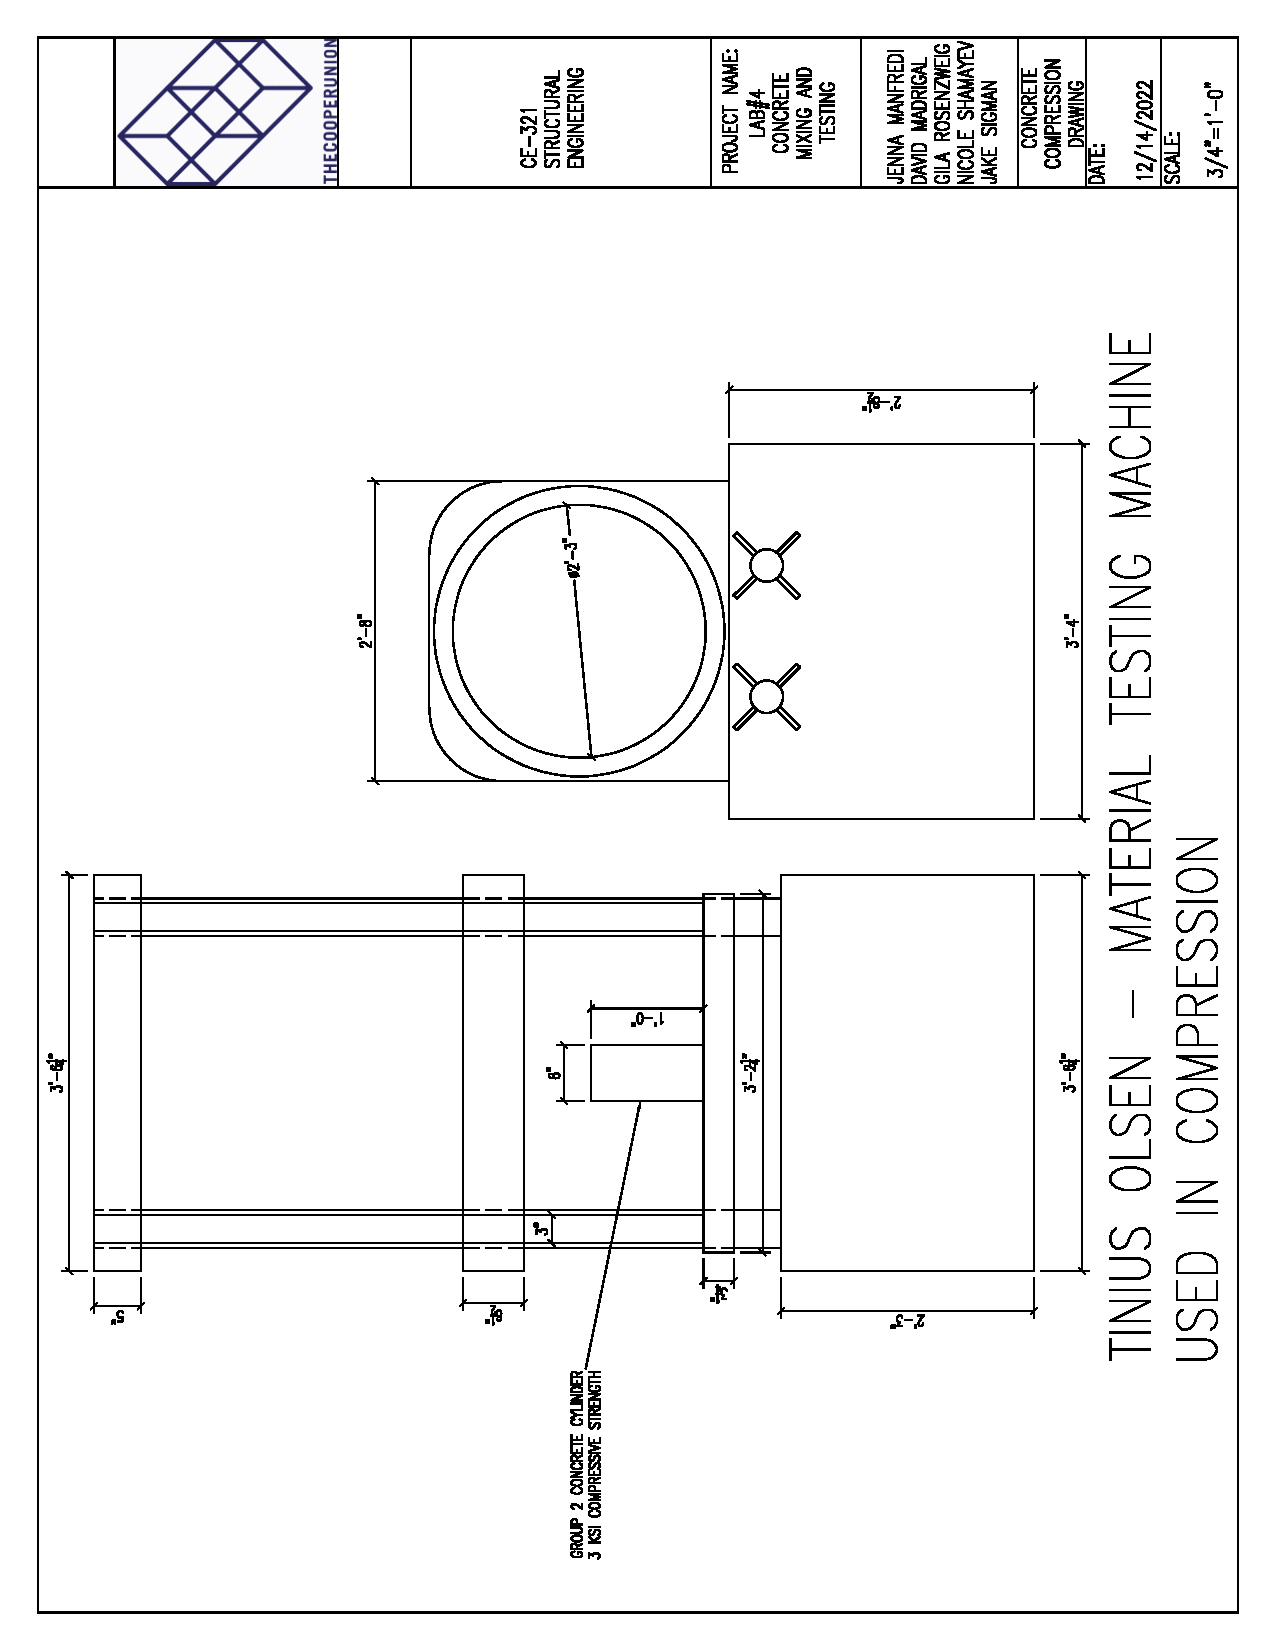
\includepdf[pages=-,pagecommand={\phantomsection\addcontentsline{toc}{subsection}{Equipment Drawing}\thispagestyle{empty}}]{dwg.pdf}
    \end{landscape}
    \newpage
    \section{Theory}
    \noindent Concrete is one of the primary building materials in construction projects. Mixtures made on-site have good plasticity that allows them to be cast into various shapes of all sizes. Concrete is also cheap as the vast majority of the raw material is sand and stone. Not only does concrete have a naturally high strength when made properly, but concrete is highly modular. For example, lighter aggregates can be used to make more economical lightweight concrete and similarly, steel rebar can be used to improve its tension strength; the function of concrete is literally modified by its form which lets it be used in almost any building project. \\\\
    In the design of concrete mixes, the \emph{absolute volume method} is the fundamental outline to calcuate the volumes of cement, water, coarse aggregate, fine aggregate, and air. Cement is a hydraulic mineral binding material; when mixed with water, a hard cement block forms and binds granulated materials together. The most common type of cement is Portland cement which is used in this experiment. In the manufacturing of Portland cement, an intermediate cement clinker is formed when limestone, clay soil, and iron ore are \emph{sintered}, or fused together without any liquefaction. When the clinker is ground with limestone and gypsum, Portland cement is formed. When hydrated, the plasticity of cement is lost with no change of strength, referred to as the \emph{setting}. This process directly determines the strength of the cement which in turn defines the strength of concrete.\\\\
    Aggregates used for ordinary concrete are defined by their size; any particle with a diameter greater than 4.75 mm is called \emph{coarse aggregate}, and a diameter smaller is considered \emph{fine aggregate}. Typically, granulated sand is used as the fine aggregate, and gravel and pebbles are used as coarse aggregates. \\\\
    The \emph{workability} of concrete is defined as how viscous, mobile, and water-retentive concrete is. Concrete that is not workable will not be able to be poured in a desirable manner. The most common determination method of workability is the \emph{slump test}, which involves pouring a fresh concrete mixture into a conical tube. The concrete will settle under its own weight and the height difference between the top of the cone and the top face of the concrete is the slump. This affects the mobility of the concrete, but the cohesion can be determined by lightly tapping the side of the cone to see if there are any cracks in the mixture. \\\\
    \begin{equation}
        f'_{cr}=\frac{P}{A}
    \end{equation}
    The compressive strength of concrete is influenced by the cement strength grade and the \emph{water-cement ratio}.  A desired compressive strength $f'_{cr}$ defines the water-cement ratio. The experimental compressive strength is calculated using Equation 1. The weight of cement should be calculated which in turn defines the bulk volume and bulk density of the mixture. This allows the ratios of sand, aggregate, and water to be known. For this laboratory experiment, a target compressive strength concrete will be mixed with calculated weights of the aggregate, water, and cement. 
    \newpage
    \section{Sample Calculations}
    \subsection{Area}
    \[A=\frac{\pi}{4}\times d^2\]
    \[A=\frac{\pi}{4}\times (\text{6 in})^2=\boxed{\text{28.27 in}^2}\]
    \subsection{Volume}
    \[V=A\times h\]
    \[V=\text{28.27 in}^2\times\text{12 in}=\boxed{\text{339.29 in}^3}\]
    \subsection{Compressive Strength}
    \[f'=\frac{P}{A}\]
    \[f'=\frac{\text{16000 lb}}{\text{28.27 in}^2}=\boxed{\text{565.88 psi}}\]
    \subsection{Error}
    \[\%_\text{Error}=\frac{|\text{Theoretical}-\text{Experimental}|}{\text{Theoretical}}\times 100\%\]
    \[\%_\text{Error}=\frac{|\text{84824 lb}-\text{16000 lb}|}{\text{84823 lb}}\times 100\%=\boxed{81.14\%}\]
    \newpage
    \section{Results}
    \noindent The desired ratios for the group's assigned compressive strength (3000 ksi) were used in accordance with the lab manual. The volume was calculated to be \(\boxed{0.196\text{ ft}^3}\). Table 1 shows the calculated weights of each ingredient for the concrete.
    \begin{center}
    \addcontentsline{lot}{table}{Table 1: Required Weights of Ingredients}
    {\large{\bf Table 1: Required Weights of Ingredients\\}}
    \vspace{3mm}
    \begin{tabular}{|cccc|}
        \hline
        \textbf{Ingredient} & \textbf{Weight at 1 \(\text{ft}^3\) (lbs)} & \textbf{Theoretical Weight (lbs)} & \textbf{Experimental Weight (lbs)}  \\\hline
        Water      & 12.6   & 2.47                               & 3.15                                 \\
        Cement     & 18.5   & 3.63                               & 4.63                                 \\
        Aggregate  & 63     & 12.37                              & 15.75                                \\
        Sand       & 52.6   & 10.33                              & 13.15                                \\\hline
    \end{tabular}
    \vspace{5mm}
    \end{center}
    In accordance with the 3000 psi desired compression strength, the theoretical value of the compressive load was calculated to be \(\boxed{\text{84823 lb}}\). However, upon compressing the concrete, it was found that the experimental value of the compressive load was \(\boxed{\text{16000 lb}}\), a compressive strength of \(\boxed{\text{565.88 psi}}\). This resulted in an error of \(\boxed{81.14\%}\).
    \newpage
    \section{Conclusion}
    \indent Concrete cylinder testing a one of the most common ways to test the compressive strength of a concrete mix and is the standard for acceptance. When cast on a job site, cylinders are not intended to represent the concrete’s in-place strength within the structure, but rather as a performance check of the mix delivered to the site. A “standard curing” process outlined by ASTM C31 / AASHTO T 23.39 that involved a controlled and protected initial curing, after which samples are retrieved for final laboratory curing within 48 hours.  There are also options for ``field curing'' for the cases where it is necessary to monitor strength development in ambient conditions at the job site; field-cured cylinders to not adhere to separate moisture and humidity requirements for initial curing. Instead, they undergo the same moisture and temperature conditions as in the structural work, with the intention that they reflect the strength development of the concrete in place.\\ 
    \indent Not much equipment is needed in the field to collect and mold samples: a wheelbarrow, to collect a composite of samples; a scoop, large enough to collect representative samples and small about to handle and place easily; specified tamping rod, appropriate to the cylinder of choice; concrete vibrator, permitted for consolidation and required when there is a slump of 1 inch or less. One test of 2 specimens is required for every 150 cubic yards of concrete, with a minimum of one test each day on a site. 
    Samples are initially cured in a controlled environment (unless they are to be field-cured) for 48 hours, and then cured in the laboratory for controlled and consistent moisture and temperature conditions. This final curing environment required removal of the mold and transfer to the curing environment immediately so there is no loss of moisture or risk of damage before the cure is complete. Prior to testing, a mixture of sulfur, fly ash, and mineral filler is applied in flowable form as a cap on the cylinder to ensure that loading will be genuinely axial. Alternatively, neoprene pads can be used to distribute load evenly, and concrete cylinder end griding can also be done to ensure square ends. \\
    \indent Upon loading, fracture type should be described and documented. There are 6 typical forms of cracks, as seen in figure 1. \\
    \begin{center}
        \addcontentsline{lof}{figure}{Figure 1: Forms of Cracks in Concrete}
        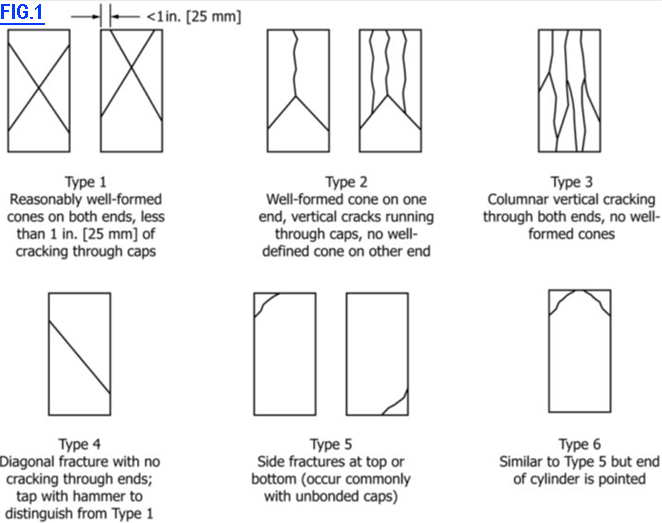
\includegraphics[scale=0.5, frame]{fig1.png}
        \\Figure 1: Forms of Cracks in Concrete\\
    \end{center}
    \par The testing done in this particular experiment was on a much smaller scale than field conditions; concrete was mixed in amounts sufficient for one cylinder. Weight ratios of the materials were calculated and mixed to form a concrete mixture. Upon loading, the cylinder broke at 16,000 lbs of force, where it was projected to reach 90,000 lbs based on design strength and surface area, experiencing Type 3 cracking, first on one half of the cylinder and then around the full circumference. The difference in cracking load gives an error of 81.14\% which is quite large. With such large error, it is especially important to consider all potential sources of error. \\
    \indent The primary source of error arises from the use of expired cement. It is easy to dismiss expiration dates, but with some products it is crucial that expiration dates be heeded. When forming the concrete mix, it was noticeable that the cement was of the wrong consistency: there were clumps rather than a very fine powder as there should have been. Additionally, it is possible that the aggregate was not soaked sufficiently, and that insufficient water was added to the mix. When the concrete broke, it had a very crumbly texture, indicating that the mix was too dry. This was also somewhat noticeable from the time of mixing, as the slump test showed a slump close to 0 inches. Other error relating to slump regards how the concrete was tamped into the cylinder. A tamping rod was used, however, in the field when concrete has such low slump, a vibrator is required to settle the concrete into the cylinder. The lack of vibrator use means it is likely there was extra air in the cylinder, which would increase how brittle the specimen was. \\
    \indent Further error, although less impactful, is the lack of use of a cap on the cylinder to ensure accurate axial loading; the surface planes of the top of the cylinder was not perfectly smooth, and thus axial loading would not be well distributed across the surface area. It is also likely that the actual proportions of water : cement : aggregate : sand were incorrect, even if the calculated proportions were correct. Such error would be attributable to how the components were measured. 
    To improve this experiment, it is important to use cement that is not yet expired and is still the appropriate texture. Additionally, it would be advisable to soak aggregates for a sufficient length of time to ensure water is not absorbed by the sand leaving insufficient amounts of water for chemical reaction. Capping the cylinders will help in distributing the loading accurately and axially so cracking is less likely to be localized on one side of the cylinder. 
    \newpage
    \section{References}
    
    \begin{description}
        \item Ferdinand B. \emph{et. al.} (2015). \emph{Mechanics of Materials}, 7th Ed., McGraw Hill, New York.
        \item Ben B. (2021). Concrete Cylinder Testing - From the Field to the Lab, \url{https://www.globalgilson.com/blog/concrete-cylinder-test#:~:text=The%20prepared%20concrete%20test%20cylinders,and%20their%20purpose%20is%20straightforward} (accessed 8 December 2022).
        \item Concrete Construction Staff (1975). Number of Test Cylinders Required, \url{https://www.concreteconstruction.net/how-to/number-of-test-cylinders-required_o#:~:text=How%20many%20test%20cylinders%20are,placed%20in%20any%20one%20day} (accessed 8 December 2022).
        \item McGraw-Hill Education Access Engineering. Concrete Mix Design (accessed 8 December 2022).
        \item Haimei Z. (2011). \emph{Building materials in civil engineering}, Woodhead Publishing, Sawston.
    \end{description}
    \newpage
    \section{Appendix}
    \begin{center}
        Cylinder Height, \(H\) (in): 12\\
        Cylinder Diameter, \(D\) (in): 6\\
        Cylinder Cross-Sectional Area, \(A\) (\(\text{in}^2\)): 28.27\\
        Cylinder Volume, \(V\) (\(\text{in}^3\)): 339.29\\
        \vspace{5mm}
        \begin{tabular}{|c|c|c|c|c|}
            \hline
            \textbf{Cement (lb)} & \textbf{Sand (lb)} & \textbf{Coarse Aggregate (lb)} & \textbf{Water (lb)} & \textbf{Water-to-Cement Ratio} \\\hline
            4.63 & 13.15 & 15.75 & 3.15 & 0.68 \\\hline
        \end{tabular}
        \vspace{5mm}
        \\Slump, \(S\) (in): 0\\
        \vspace{5mm}
        \begin{tabular}{|l|c|c|}
            \hline
            & \textbf{Theoretical} & \textbf{Experimental} \\\hline
            \textbf{28-Day Compressive Load \(\bm{P_{28}}\), (lb)} & 84823 & 16000 \\
            \textbf{28-Day Compressive Load \(\bm{f_{\textbf{c28}}'}\), (psi)} & 3000 & 565.88 \\\hline
        \end{tabular}
        \vspace{5mm}
        \\28-Day Compressive Strength Error, Error \(f_{\text{c28}}'\) (\%): 81.14
    \end{center}
\end{document}